\begin{answer}
\begin{figure}[H]
    \centering
    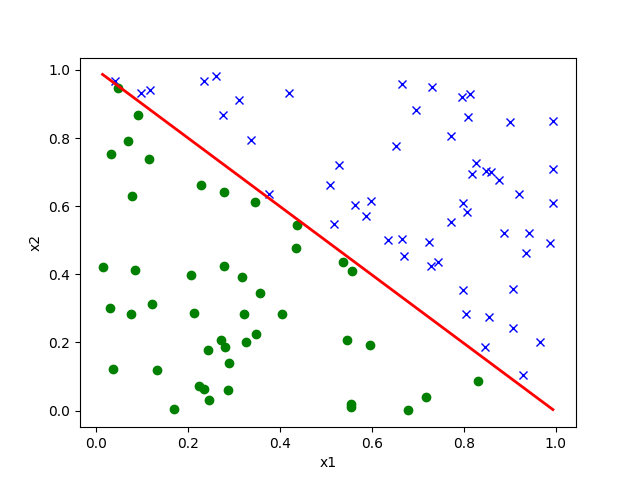
\includegraphics[width=9cm]{logreg_stability/logreg_pred_b.png}
    \caption*{Logistic regression decision boundary on dataset B}
\end{figure}
\begin{figure}[H]
  \centering
  \begin{subfigure}[b]{0.49\textwidth}
    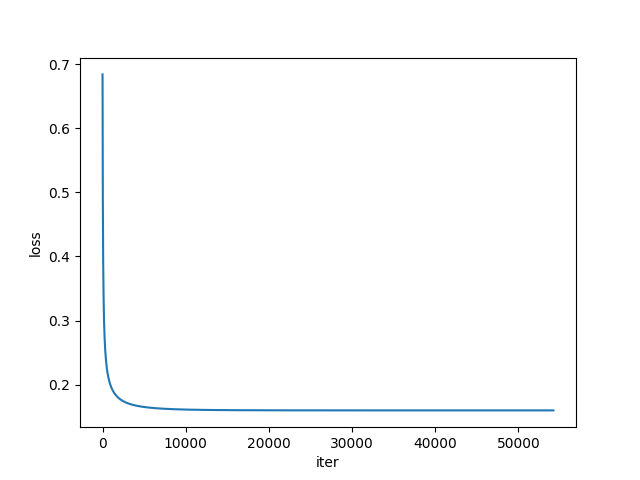
\includegraphics[width=\textwidth]{logreg_stability/logreg_pred_a_loss.png}
    \caption*{Loss by iteration on dataset A}
  \end{subfigure}
  \begin{subfigure}[b]{0.49\textwidth}
    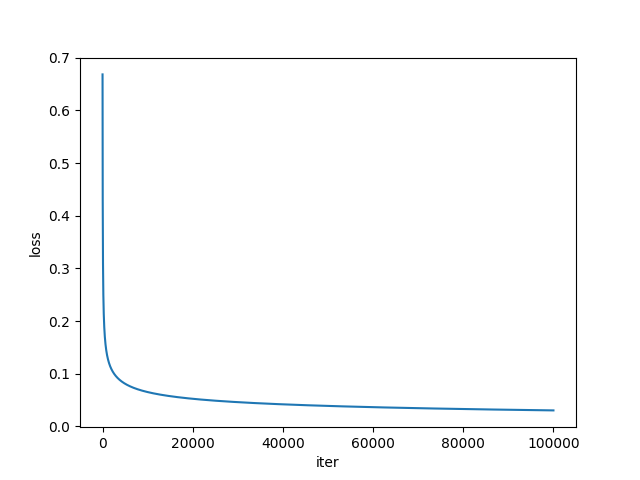
\includegraphics[width=\textwidth]{logreg_stability/logreg_pred_b_loss.png}
    \caption*{Loss by iteration on dataset B}
  \end{subfigure}
\end{figure}
From the decision boundary plot, we observe that dataset B is linearly separable, however by a very small margin. Therefore the the gradient descent doesn't converge, that is due to the weights increasing in magnitude(norm) as the model overfits(model gets overconfident). This phenomenon is displayed on the following plot.
\begin{figure}[H]
  \centering
  \begin{subfigure}[b]{0.49\textwidth}
    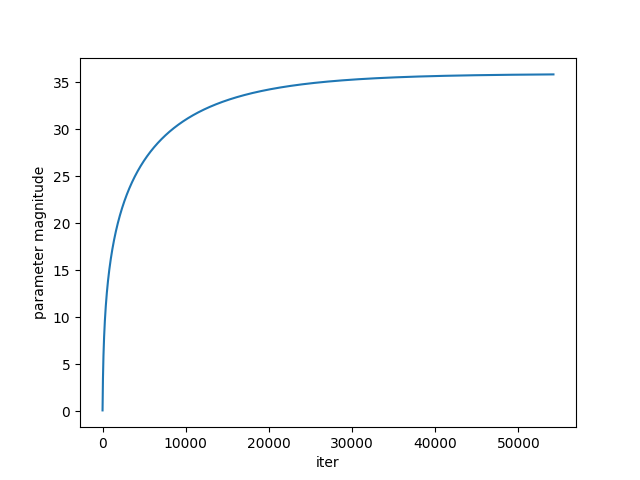
\includegraphics[width=\textwidth]{logreg_stability/logreg_pred_a_param_magnitude.png}
    \caption*{Magnitude of weights for model A}
  \end{subfigure}
  \begin{subfigure}[b]{0.49\textwidth}
    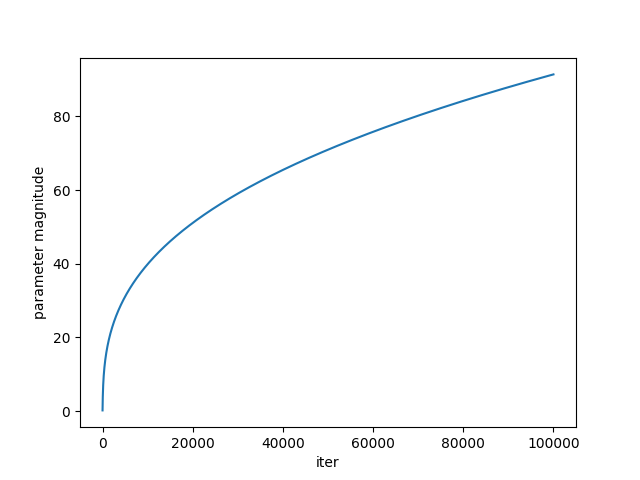
\includegraphics[width=\textwidth]{logreg_stability/logreg_pred_b_param_magnitude.png}
    \caption*{Magnitude of weights for model B}
  \end{subfigure}
\end{figure}
On the plot, we see that the norm of the weights of model B tend to infinity with more iterations.
\end{answer}
